\section{Desenvolvimento}\label{sec:desenvolvimento}

\begin{frame}{Recursos Necessários}
	\begin{itemize}
		\setlength{\itemsep}{1em}
		\item<1-> Protégé
		\item<1-> Android Studio
		\item<1-> SQLite
		\item<1-> Apache Jena
		\item<1-> Trello
	\end{itemize}
\end{frame}

\subsection{Ontologia}
\begin{frame}{A Ontologia}
	\begin{itemize}
		\setlength{\itemsep}{1em}
		\item<1-> Baseada na ontologia de pizza de Standford
		\item<1-> Classes de \textit{ingredientes} e \textit{produtos}
		\item<1-> Propriedades:
		\begin{itemize}
			\setlength{\itemsep}{0.5em}
			\item<1-> Ingredientes
			\item<1-> Preço
			\item<1-> Restrições alimentares: \\ 
			\vspace{-0.5em}
			\begin{minipage}[t]{0.4\linewidth}
				\begin{itemize}
					\setlength{\itemsep}{0.5em}
					\item<1-> Se possui glúten
					\item<1-> Se possui lactose
					\item<1-> Se é vegetariano	
				\end{itemize}
			\end{minipage}
			\begin{minipage}[t]{0.4\linewidth}
				\begin{itemize}
					\setlength{\itemsep}{0.5em}
					\item<1-> Nível de sal
					\item<1-> Nível de gordura			
				\end{itemize}
			\end{minipage}
			\item<1-> Se é um produto contável ou não
		\end{itemize}
	\end{itemize}
\end{frame}

\begin{frame}[b]{Integração da Ontologia}
	\begin{tikzpicture}[overlay]
		\node<1-1> (A) at (5,3.22) {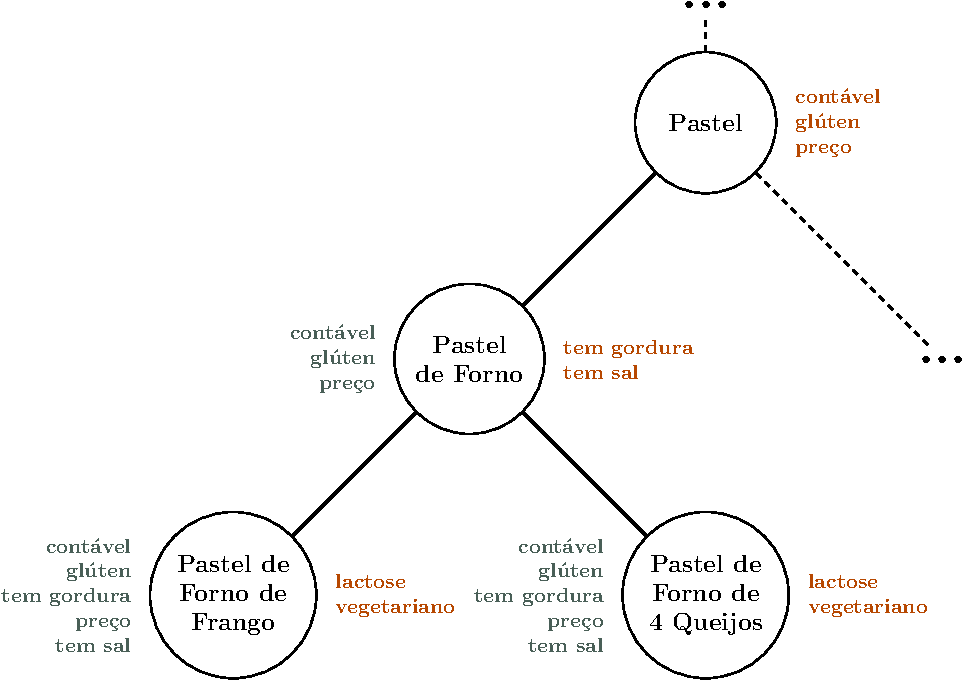
\includegraphics[width=0.8\linewidth]{../pdf/tikz/toptop-1.pdf}};
		\node<2-2> (A) at (5,3.22) {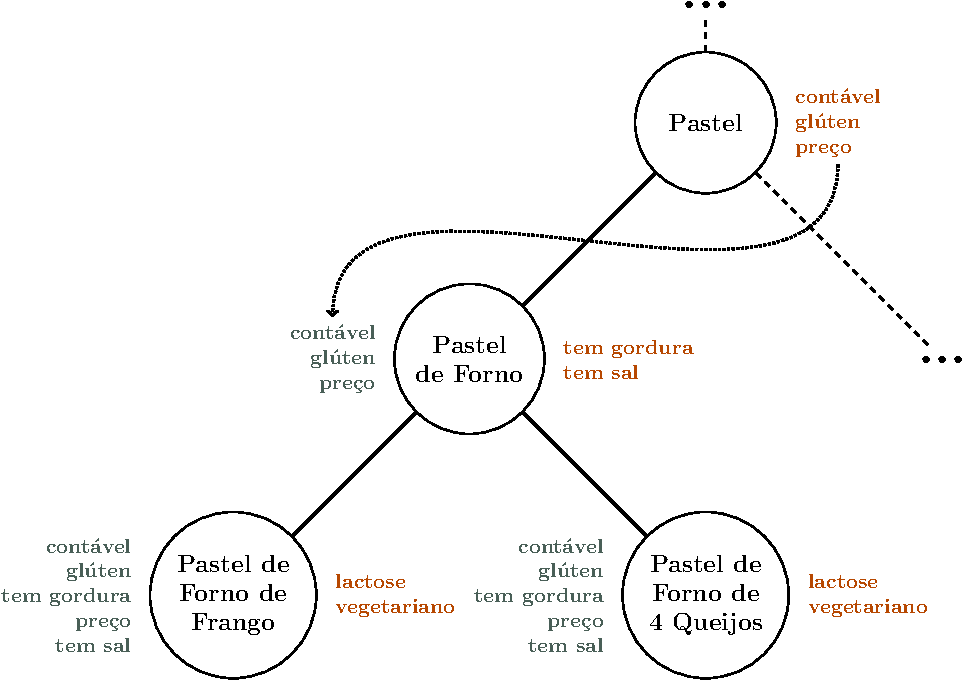
\includegraphics[width=0.8\linewidth]{../pdf/tikz/topdown-1.pdf}};
		\node<3-3> (A) at (5,3.22) {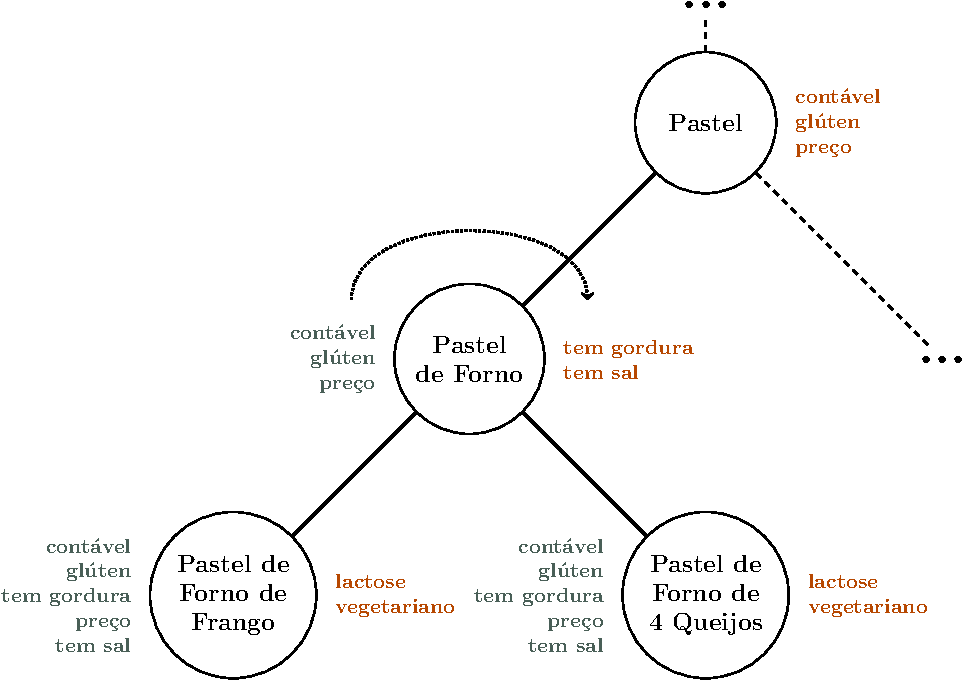
\includegraphics[width=0.8\linewidth]{../pdf/tikz/topdown-2.pdf}};
		\node<4-4> (A) at (5,3.22) {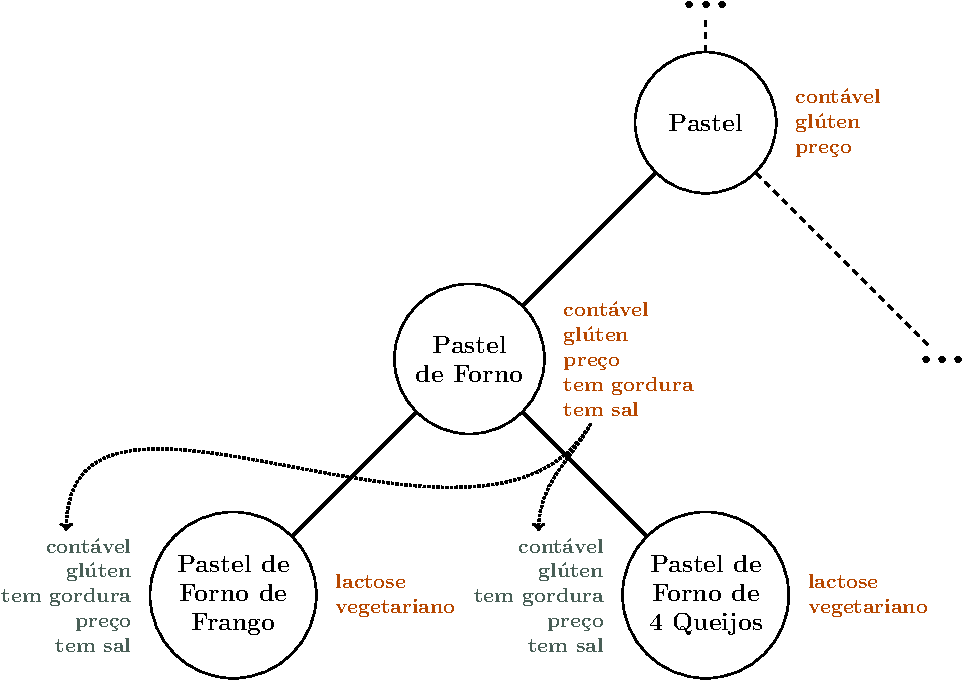
\includegraphics[width=0.8\linewidth]{../pdf/tikz/topdown-3.pdf}};
		\node<5-5> (A) at (5,3.22) {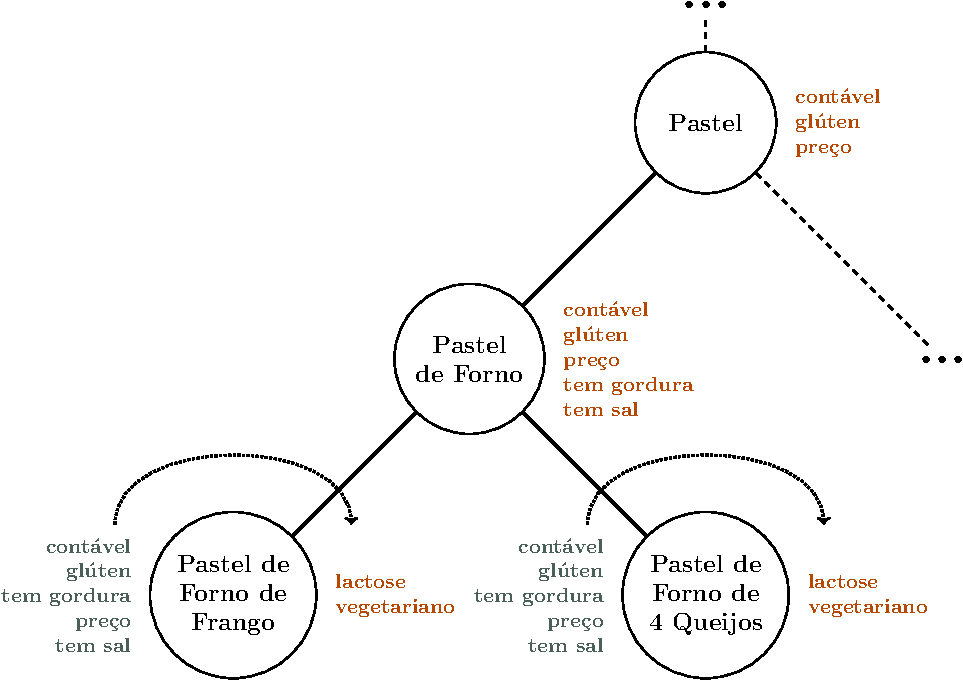
\includegraphics[width=0.8\linewidth]{../pdf/tikz/topdown-4.pdf}};
		\node<6-6> (A) at (5.67,3.22) {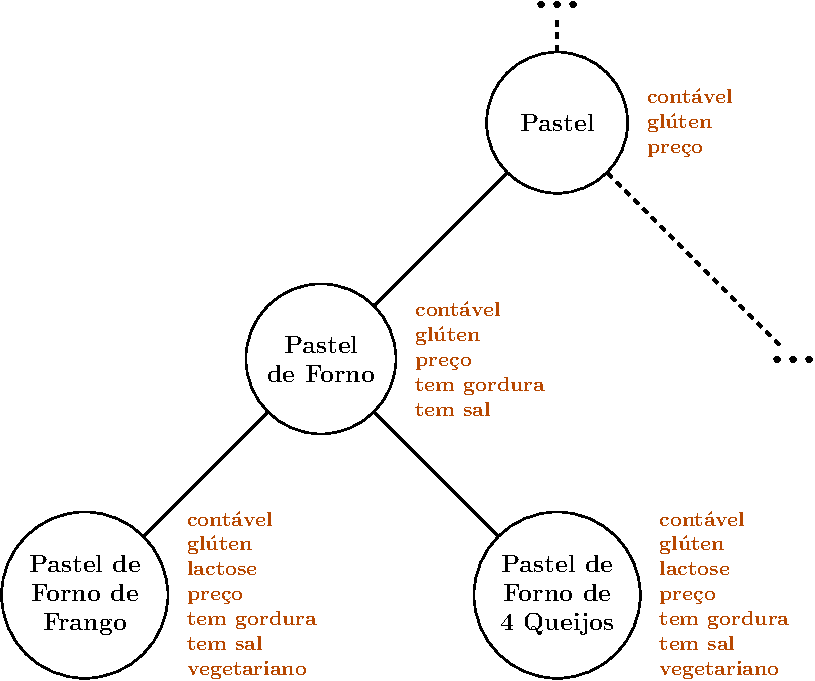
\includegraphics[width=0.676\linewidth]{../pdf/tikz/topdown-5.pdf}};
		\node<7-7> (A) at (5.67,3.22) {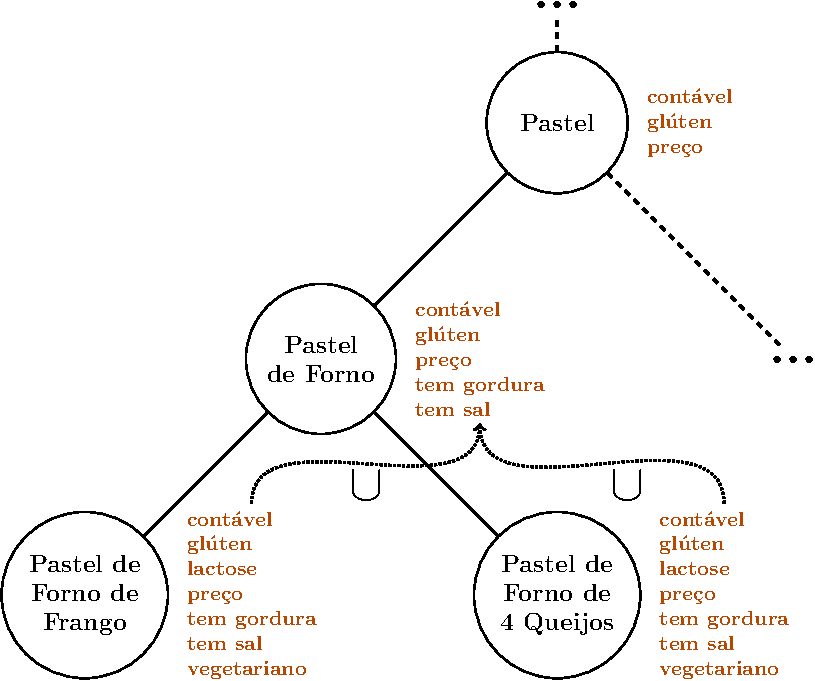
\includegraphics[width=0.676\linewidth]{../pdf/tikz/bottomup-1.pdf}};
		\node<8-8> (A) at (5.67,3.22) {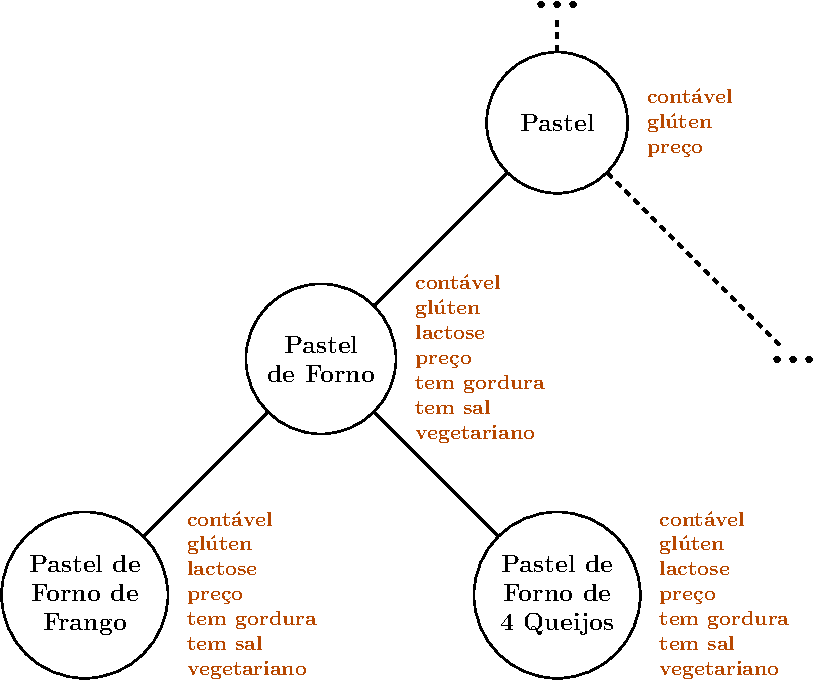
\includegraphics[width=0.676\linewidth]{../pdf/tikz/bottomup-2.pdf}};
		\node<9-9> (A) at (5.67,3.22) {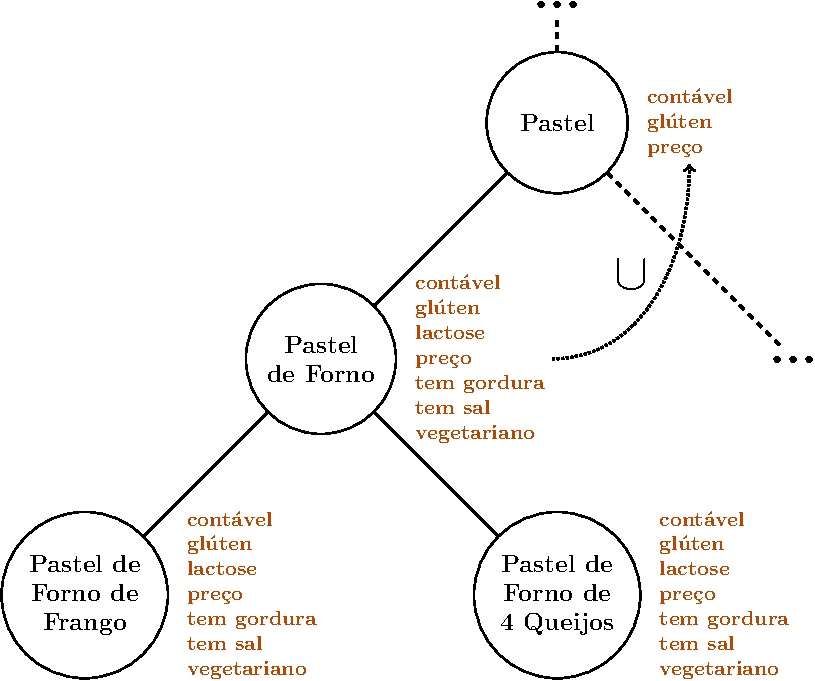
\includegraphics[width=0.676\linewidth]{../pdf/tikz/bottomup-3.pdf}};
		\node<10-10> (A) at (5.67,3.22) {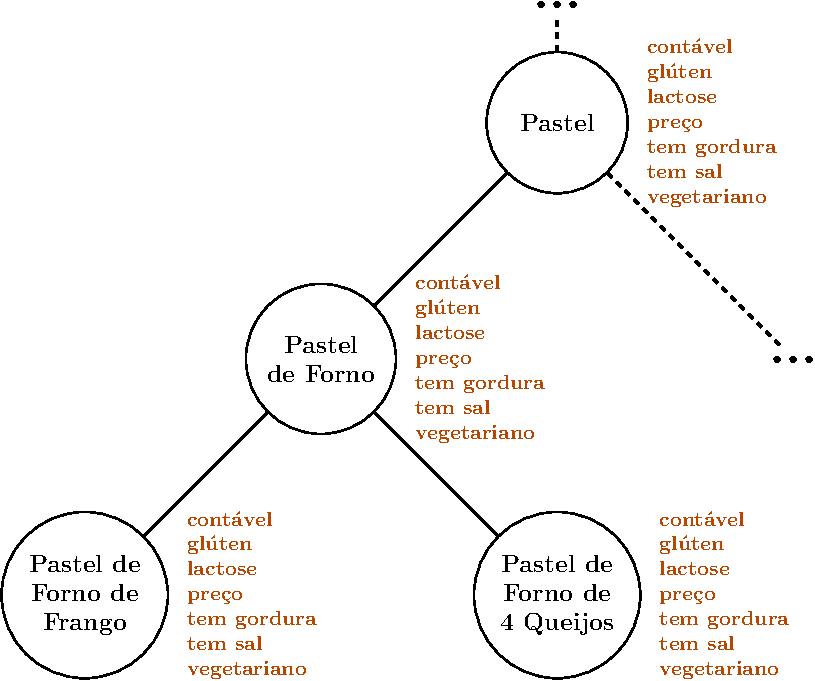
\includegraphics[width=0.676\linewidth]{../pdf/tikz/bottomup-4.pdf}};
		\node<11-11> (A) at (5.67,3.6) {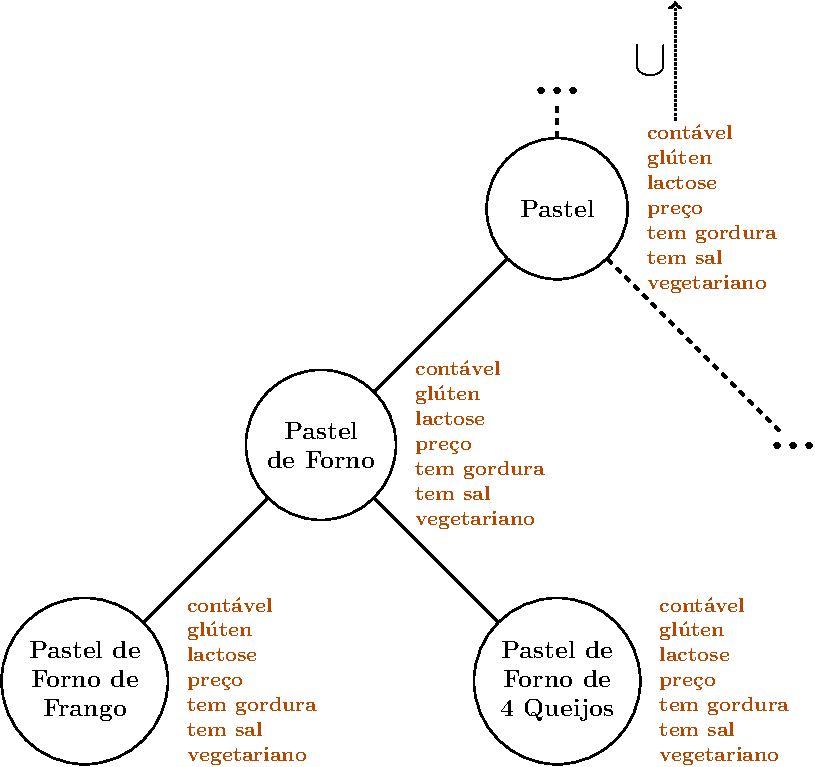
\includegraphics[width=0.676\linewidth]{../pdf/tikz/bottomup-5.pdf}};
	\end{tikzpicture}
\end{frame}